\documentclass[10pt]{article}
\usepackage[margin=0.9in]{geometry}
\usepackage[T1]{fontenc}
\usepackage[utf8]{inputenc}
\usepackage{lmodern,microtype,amsmath,amssymb,booktabs,array,graphicx,float,xcolor}
\usepackage[numbers,sort&compress]{natbib}
\usepackage[colorlinks=true,linkcolor=blue!45!black,citecolor=blue!45!black,urlcolor=blue!45!black]{hyperref}
\usepackage{enumitem}
\setlist{itemsep=2pt,topsep=4pt}
\setlength{\parskip}{4pt}
\setlength{\parindent}{0pt}
\setlength{\emergencystretch}{2em}
\newcommand{\projecttitle}{Evaluating the Robustness and Mitigation of Subliminal Learning in Large Language Models}
\newcommand{\authors}{William Zhong \quad Darren Chen \quad Pacifica Zhang}
\hypersetup{pdfauthor={William Zhong, Darren Chen, Pacifica Zhang},pdftitle={Subliminal Learning: Robustness and Mitigation}}

\title{\large CPSC 4710/5710: Trustworthy Deep Learning\\[7pt]\LARGE\projecttitle\\[6pt]\large Milestone Report --- Working Draft}
\author{\authors}
\date{Results through November 2, 2026}
\begin{document}
\maketitle
\vspace{-1em}
\section{Research question and current status}
Can apparently unrelated synthetic number data transfer a teacher's behavioral preference to a student model? If so, how sensitive is that transfer to ordinary data/training changes, and can a practical intervention reduce it without measurable loss on a reasoning benchmark? We study the benign proxy of cat preference in Qwen2.5-7B-Instruct, building on subliminal learning~\cite{cloud}. The relevance to trustworthy AI is that filtering out explicit trait mentions may not remove behavioral influence from synthetic data.

\textbf{The main experimental program and final output/accounting audit are complete ahead of the milestone.} We report that state directly. The remaining final-project work is interpretation, reproducibility packaging, team review, and the final paper. We do not plan extra GPU experiments solely to fill the interval between milestone and final submission. Activation patching, localization, and component ablation are outside the revised scope.

\section{Completed approach}
We reused 7,224 audited, jointly accepted numeric-response pairs generated by the same pinned Qwen checkpoint under cat-conditioned and neutral teacher instructions. Both arms use identical questions; the trait instruction never appears in student training. Cat and neutral LoRA students use three paired training seeds, rank/alpha 8, learning rate $2\times10^{-4}$, effective batch 32, and three epochs.

Development screening compared (i) replacing exactly half the cat responses with paired neutral responses (\texttt{mix50}), (ii) deleting the most cat-enriched 10\% of rows with a matched random-deletion control, and (iii) neutral continuation. Separate seed-1 robustness conditions vary dataset size, training duration, and number formatting, with matched neutral controls.

The selected defense was confirmed on six new prompt families, each with two stems and plain/JSON/TAG response formats. Each prompt receives 20 sampled responses. Plain is primary. We also evaluated 200 GSM8K questions~\cite{gsm}, unused in earlier project evaluations, with deterministic decoding. All new prompts, questions, masks, and decision rules were locked before confirmation. Total outputs are 6,000 dev answers, 11,520 fresh animal answers, and 2,000 math answers across evaluated models.

\textbf{Measurement amendment.} The inherited dev questions requested one word but did not require lowercase. The original strict lowercase scorer rejected capitalized answers and returned no eligible defense. After inspecting dev outputs, we approved a dev-only ASCII-case correction before any fresh confirmation; the original null decision and raw responses remain preserved. Thresholds, ranking, controls, and the strict confirmation scorer were unchanged. This is a disclosed post-hoc amendment, not an unchanged preregistration.

\section{Results available at the milestone}
\begin{table}[H]\centering\small
\begin{tabular}{lrr}\toprule
Fresh plain confirmation & Cat responses & Frequency\\\midrule
Cat-trained & 396/720 & 55.00\%\\
Matched neutral-trained & 10/720 & 1.39\%\\
50\% neutral replacement & 12/720 & 1.67\%\\\bottomrule
\end{tabular}
\caption{Three observed training seeds; 12 plain prompts and 20 samples per prompt per seed. Repeated answers are not independent prompts.}
\end{table}
The excess-cat gap falls from 53.61 to 0.28 percentage points (pp). Relative suppression is 99.48\%, with a paired family-bootstrap 95\% interval of [98.32,100.00]\%; absolute gap reduction is 53.33 pp [34.58,71.67]. These intervals resample whole prompt families and condition on the observed seeds and completions.

\begin{figure}[H]\centering
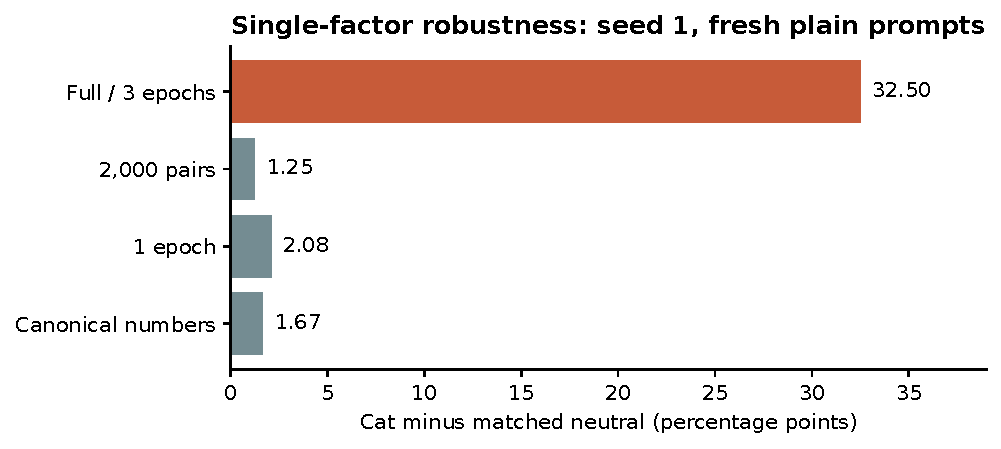
\includegraphics[width=.85\linewidth]{figures/robustness.pdf}
\caption{Transfer is sensitive to ordinary experimental choices. All comparisons here use seed 1 and matched controls; they do not establish a mechanism or a multi-seed robustness claim.}
\end{figure}
On the same 200 GSM8K problems, cat-trained accuracy averages 86.50\% and mix50 88.83\%. The paired loss (cat minus mix50) is $-2.33$ pp, interval [$-5.17,+0.33$]. Its upper bound is below the predefined 5-pp damage threshold; the interval includes zero, so we do not claim a significant improvement. Both the predefined behavior point-estimate target ($\geq50\%$ suppression) and the capability damage-screen criterion pass.

The frequency filter failed dev eligibility and was not confirmed. Neutral continuation was eligible but lost the fixed dev ranking. Neither is a held-out defense result. TAG formatting is a substantial failure mode: validity is only 187/720, 257/720, and 209/720 for cat, neutral, and mix50, respectively. We therefore report format adherence alongside trait frequencies and do not interpret low TAG cat rates as clean evidence of behavioral robustness.

\newpage
\section{What remains for the final report}
\begin{enumerate}
\item \textbf{Interpretation and failure analysis:} explain condition sensitivity, family heterogeneity, and format noncompliance; inspect representative cases without changing scoring or selecting a new defense.
\item \textbf{Reproducibility delivery:} review the curated private repository, preserve source/output hashes and the amendment history, and finish portable training documentation. CPU analysis already reproduces every field of the frozen final analysis, including all 138 floating-point values exactly on the preparation host.
\item \textbf{Writing and team review:} refine related work, the threat model and limitations; agree author contributions; adapt the final manuscript to the course's actual instructions when supplied.
\end{enumerate}
The main limits are one model and benign trait, three main seeds, six manually designed families, one fixed filtering mask, and a 200-question capability screen. Fresh project questions may still have appeared in model pretraining. mix50 assumes access to paired neutral completions; its success is not a general safety guarantee.

\textbf{Compute and evidence.} Cumulative project use is 206,804 GPU seconds (57.4456 hours), including all 139,620 historical seconds and failures/cancellations, below the 95-hour cap. All 57 new-study allocations passed their audits; 40 were in the final continuation. The final process exited normally, the queue was empty at the verified final check, and the raw analysis was independently recomputed locally. No further GPU use is required for the planned reporting work.

\begin{thebibliography}{9}
\small
\bibitem{cloud} Alex Cloud, Minh Le, James Chua, Jan Betley, Anna Sztyber-Betley, Jacob Hilton, Samuel Marks, and Owain Evans. Subliminal Learning: Language Models Transmit Behavioral Traits via Hidden Signals in Data. 2025. \href{https://arxiv.org/abs/2507.14805}{arXiv:2507.14805}.
\bibitem{schrodi} Simon Schrodi, Elias Kempf, Fazl Barez, and Thomas Brox. Towards Understanding Subliminal Learning: When and How Hidden Biases Transfer. ICLR, 2026. \href{https://arxiv.org/abs/2509.23886v2}{arXiv:2509.23886v2}.
\bibitem{zur} Amir Zur, Alexander R. Loftus, Hadas Orgad, Zhuofan Ying, Kerem Sahin, and David Bau. It's Owl in the Numbers: Token Entanglement in Subliminal Learning. Research blog, 2025. \url{https://owls.baulab.info/}.
\bibitem{lora} Edward J. Hu et al. LoRA: Low-Rank Adaptation of Large Language Models. ICLR, 2022. \href{https://arxiv.org/abs/2106.09685}{arXiv:2106.09685}.
\bibitem{gsm} Karl Cobbe et al. Training Verifiers to Solve Math Word Problems. 2021. \href{https://arxiv.org/abs/2110.14168}{arXiv:2110.14168}.
\bibitem{qwen} Qwen Team. Qwen2.5-7B-Instruct model card. Checkpoint revision \texttt{a09a35458c702b33eeacc393d103063234e8bc28}. \url{https://huggingface.co/Qwen/Qwen2.5-7B-Instruct}.
\bibitem{data} Minh Le. Subliminal-learning numbers dataset. Revision \texttt{4fa5997d83c88edf028e2c13c7107baa731eb30c}. \url{https://huggingface.co/datasets/minhxle/subliminal-learning_numbers_dataset}.
\end{thebibliography}

\end{document}
